\graphicspath{{./figures}}

\section{Range}

Line-of-sight range tests were conducted. Both antennas were manually positioned, and the PQ dipole was placed both horizontally and vertically. All measurements were done at the designed parameters i.e. SF 8, CR 4/6 and 500 kHz. The resulting \textit{received signal strength indicator} (RSSI) and signal-to-noise (SNR) ratio was recorded. For the unfamiliar reader, the best theoretical RSSI is 0 dB, and the minimum SNR for SF 8 is -10 dB.

Tests were done in locations around the Western Cape up until $\SI{122}{km}$, as described in Appendx \ref{sec:appendix_range}. The first test (not listed) was a 300 m test on Coetzenburg field in Stellenbosch. The link performance was found to be low compared to subsequent tests, with a recorded RSSI of -92 dBm. It is assumed that ground bounce was the major contributing factor.

\begin{figure}[!htb]
  \begin{minipage}{0.49\textwidth}
    \centering
    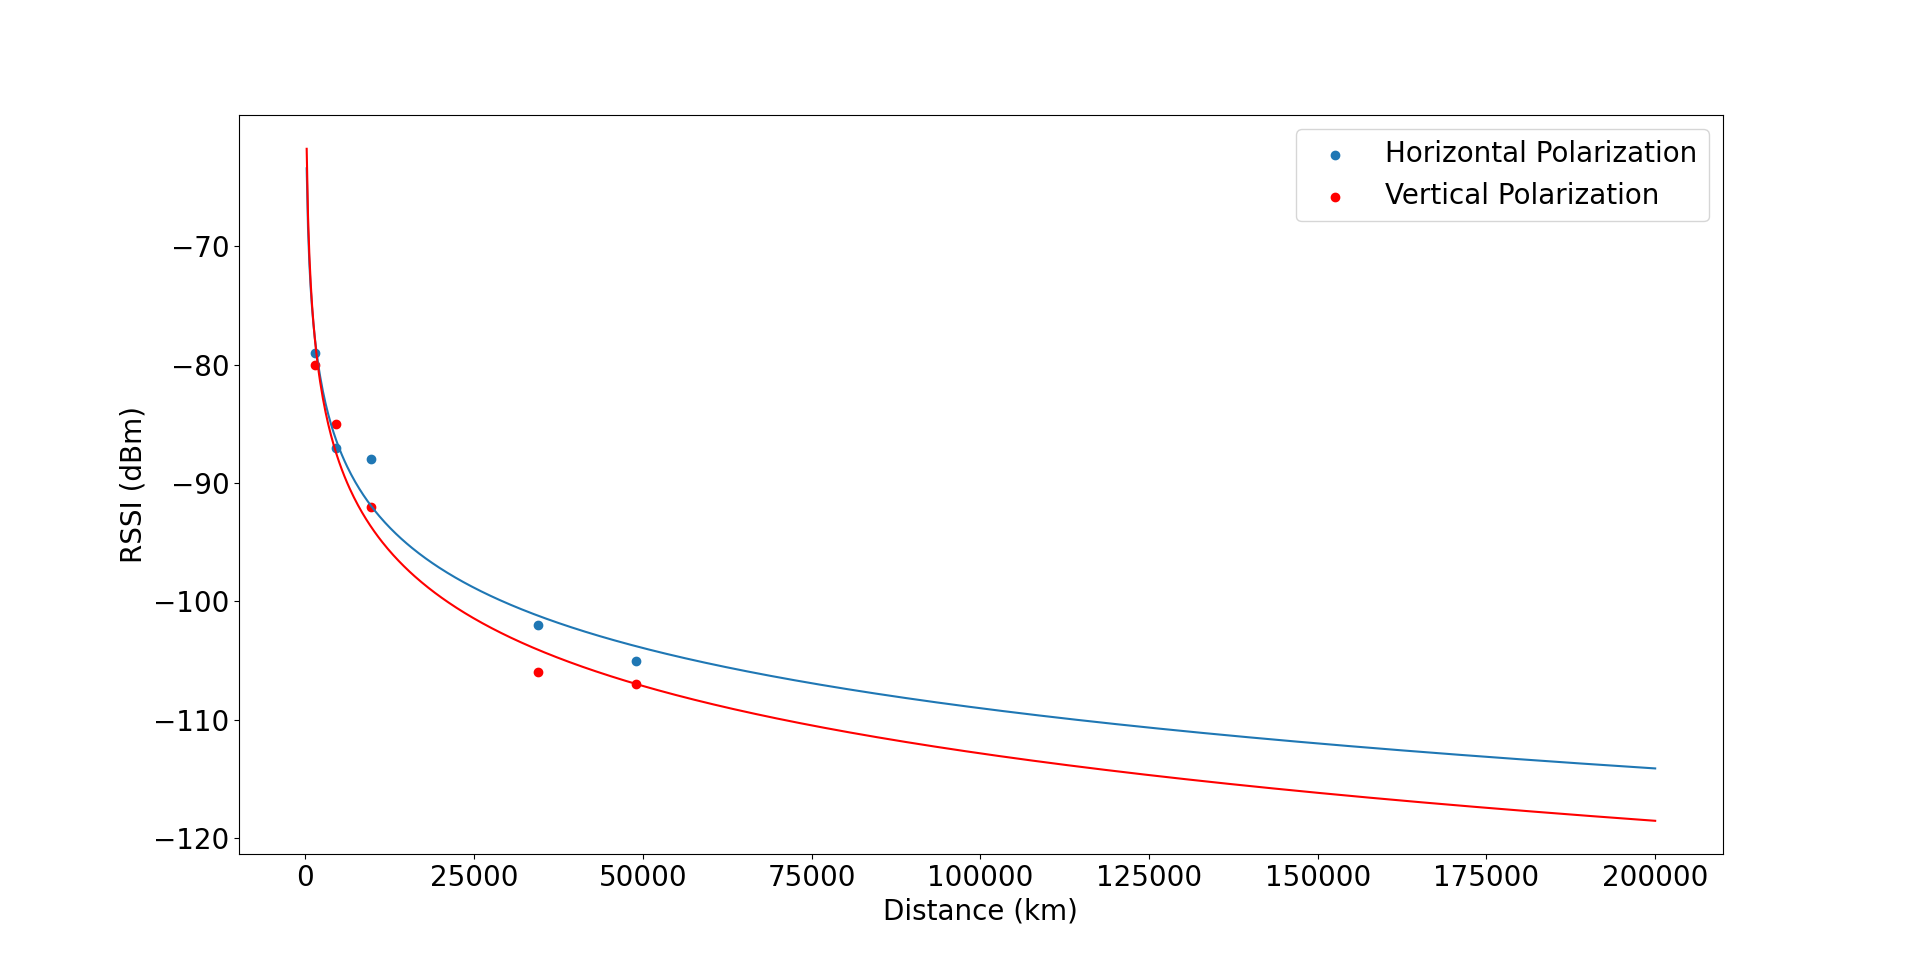
\includegraphics[width=0.99\linewidth]{rangeRssi}
    \caption{Measured RSSI vs Distance}
    \label{fig:rangeRssi}
  \end{minipage}
  \begin{minipage}{0.49\textwidth}
    \centering
    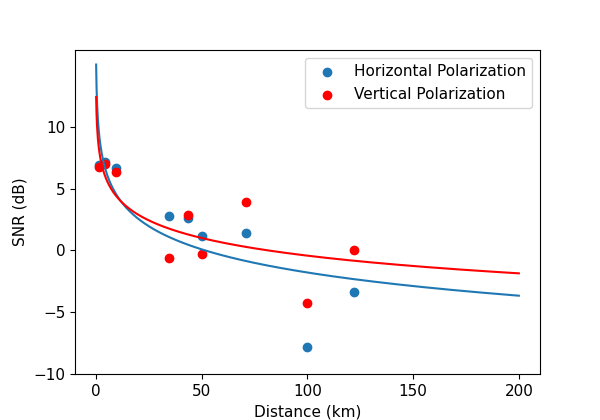
\includegraphics[width=0.99\linewidth]{rangeSnr}
    \caption{Measured SNR vs Distance}
    \label{fig:rangeSnr}
  \end{minipage}
\end{figure}

The results for the rest of the tests are plotted in Figures \ref{fig:rangeRssi} and \ref{fig:rangeSnr}, with a logarithmic curve fit. The packet contents were verified using an ID, the transmitted GPS location, and by inspecting whether a CRC (Cyclic Redundancy Check) error had occurred. The system successfully met the 120 km range requirement, and a reliable link was established at the final test of 122 km, with a recorded RSSI of -108 dBm for the vertically polarized case. Although the SNR appears to be adjusted by the receiver at closer distances, the RSSI appears to follow a logarithmic curve well, as predicted by the free space path loss formula. All tests also achieved a 100\% packet reception rate once in steady-state. For the required distance, at a sensitivity of -119 dBm, this indicates an 11 dB margin, which is slightly less than the final designed value of 12.8 dB. It is clear that the 100 km is an outlier, and it is assumed that this was due to strong multi-pathing effects caused by the transmitter being sub-optimally placed, with a large rock directly behind it. 